% default font size and doc type
\documentclass[12pt]{article}

% extra packages to bring in
\usepackage{latexsym}
\usepackage{graphicx}      % extended graphics package
\usepackage{epsfig}        % wrapper for graphicx package
\usepackage{times}
\usepackage{url}
\usepackage{listings}
\usepackage{subcaption}

% margin settings borrowed from Dr. Teresco's example paper
\setlength{\topmargin}{-0.5in}
\setlength{\textheight}{9in}
\setlength{\oddsidemargin}{0in}
\setlength{\evensidemargin}{0in}
\setlength{\textwidth}{6.5in}

% single-space command borrowed from example paper
\newcommand{\singlespace}{
  \protect\renewcommand\baselinestretch{1.0}
  \protect\normalsize
}

% 1.5 spacing borrowed from example paper
\newcommand{\doublespace}{
  \protect\renewcommand\baselinestretch{1.5}
  \protect\normalsize
}


% begin typing document
\begin{document}

% remove date
\date{}

% paper title
\title{A Behavioral Approach to 6502 Emulation
\footnote{This work was completed in partial fulfillment of the final
project requirement for Computer Science 330 at Siena College, Fall 2020.}}

\author{M.~J.~Coppola, N.~S.~Shelby, L.~E.~Carleton\\
Computer Science 330\\
Siena College\\
Loudonville, NY, 12211
}

% make title
\maketitle
% remove page number from front page
\thispagestyle{empty}

% Abstract
\begin{abstract}
%The RP2A03 is the CPU found in the Nintendo Entertainment System (NES), launched October 18th, 1985.
%This processor was based off the MOS Technology 6502, differences being a lack of a decimal mode
%and the inclusion of the Audio Processing Unit (APU). Our goal is to create a partial implementation
%of an emulator for this CPU designed to be easily extended to a simple NES emulator.
An abstract goes here. We made a 6502 emulator that was partially implemented and easy to extend.
there were some results and we're really proud. Or something along those lines.
\end{abstract}

% double spacing
\doublespace
\section{Overview}
\label{sec:overview}
The RP2A03 is the CPU found in the Nintendo Entertainment System (NES), launched October 18th, 1985~\cite{nesdev_CPU, wikipediaNES}.
This processor was based off the MOS Technology 6502, differences being a lack of a decimal mode
and the inclusion of the Audio Processing Unit (APU)~\cite{nesdev_CPU}. Our goal is to create a partial implementation
of an emulator for this CPU designed to be easily extended to a simple NES emulator. 

The emulator was designed with the NES in mind. That being said, we only emulate the behavior of
the 6502, not precicely the actual hardware. This serves us a huge simplification in implementation.
Official operations of the 6502 only need to be calculated, and not emulated. We opted in for calculating
the output of the operations immediately, and then waiting the number of clock cycles that operation
took to execute.

Overview to be continued...

\section{Bitwise Operations}
\label{sec:bitwise}

Bitwise operations are major aspect of making an efficient emulator. Supose we have an 8-bit value.
We typically express this value as a number, or possibly two hexidecimal digits. One way the 6502 uses
8-bit numbers is by defining parts of the binary expression as flags or smaller width values, shown in figure~\ref{fig:figure1}.
In emulation, it's important that we can extract information from this 8-bit number, as well as convert
information we already have into information we can store into this number. To achive this, we use
bitwise operations.

% load figures
\begin{figure}[b!]
	\centering
	\begin{subfigure}[b]{0.5\linewidth}
		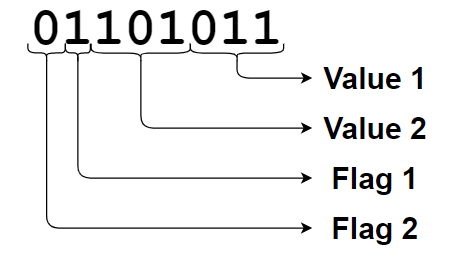
\includegraphics[width=\linewidth,bb=0 0 462 262]{figure1.PNG}
		\caption{A single binary value representing multiple values.}
		\label{fig:figure1}
	\end{subfigure}
	\begin{subfigure}[b]{0.5\linewidth}
		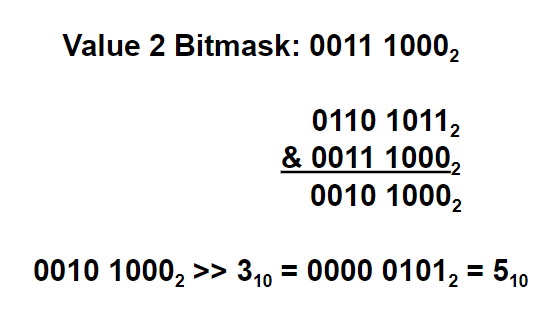
\includegraphics[width=\linewidth,bb=0 0 554 320]{figure2.PNG}
		\caption{Using a bitmask to extract values from a binary number.}
		\label{fig:figure2}
	\end{subfigure}
\end{figure}


To extract information from a binary number, we would first need to isolate that information. We can
achieve this by using a bitmask. We can create a bitmask by creating a new 8-bit number that has
1's placed over the important digits, and 0's on digits that are not. With this mask, we can use a
bitwise AND operation ( \lstinline{&} ) and have a result that only includes the digits defined by the bitmask shown in figure~\ref{fig:figure2}~\cite{bitmasks}.

Inorder to make this value useful to us, we may have to then use a bitwise shift-left ( \lstinline{>>} ) to push
the important digits to the least signifigant order of the digit. By doing this, the entirety of the
resulting 8-bit value numerically represents the value stored in the section of the original 8-bit
value~\cite{bitmasks}.

A similar process is used for setting bits as well. We create a bitmask for the bits we want to set
and or it with our value. To unset, we can \lstinline{&} with the inverse ( \lstinline{~} ) of our mask.
We can toggle/flip bits with a mask that is XOR'd ( \lstinline{^} ) with our value.

\singlespace

\bibliographystyle{abbrv}
\bibliography{references}

% end document
\end{document}
